\documentclass[12pt]{article}

\usepackage{enumerate}
\usepackage{amsmath}
\usepackage{amsthm}
\usepackage{amssymb}
\usepackage{changepage}
\usepackage{graphicx}
\usepackage[a4paper, margin=1in]{geometry}
\allowdisplaybreaks[1]

\title{DATA315 Assignment 3}
\author{Rin Meng 51940633}
\date{\today}

\begin{document}

\maketitle

\begin{enumerate}
    \item
    \begin{enumerate}
    \item
    \begin{verbatim}
source("nickel.R")
acf(nickel, lag.max = 10, 
main = "ACF of Electroless Nickel Concentrations")
     \end{verbatim}
    \begin{center}
        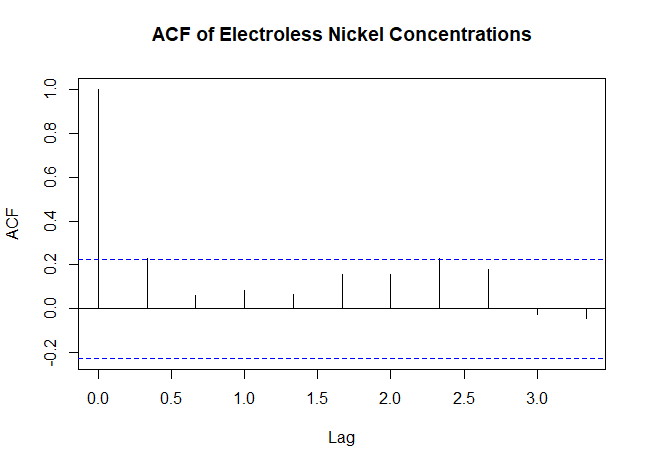
\includegraphics[width=0.8\textwidth]{Rplot.png}
    \end{center}
    The ACF plot seems to follow an MA(1) process,
    as significant correlation at lag 1 followed by immediate drop to near zero. 
    \item
\begin{verbatim}
data(lynx)
acf(lynx, lag.max = 10, main = "ACF of Lynx Trapping Data")
\end{verbatim}
    \begin{center}
        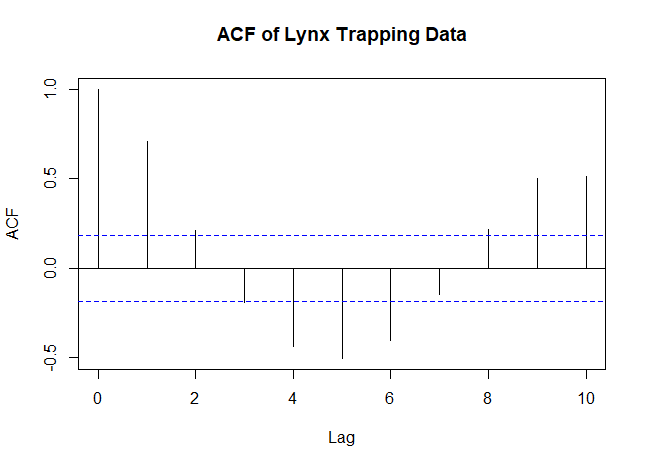
\includegraphics[width=0.8\textwidth]{Rplot01.png}
    \end{center}
    So far, there are no models that fit, because the plot shows a cyclic pattern between
    predator and prey populations. 
    \item
\begin{verbatim}
source("Globaltemps.R")
temps <- ts(temps, start = 1880, end = 2016)
acf(temps, lag.max = 10, 
main = "ACF of Global Average Temperatures")
\end{verbatim}
    \begin{center}
        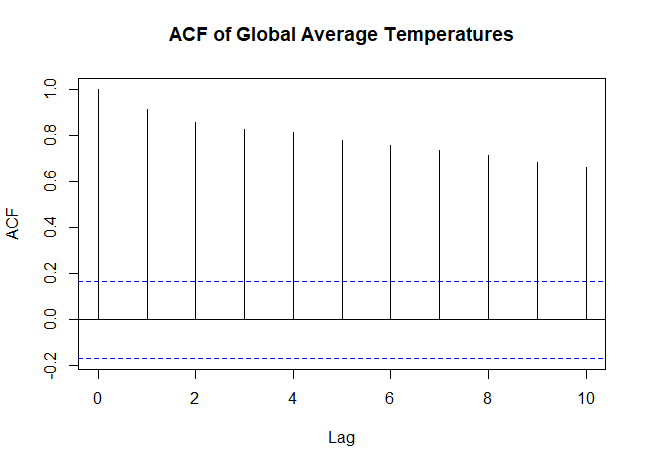
\includegraphics[width=0.8\textwidth]{Rplot02.png}
    \end{center}
    The ACF plot seems to follow an AR(1) process,
    as significant correlation at lag 1 followed by gradual decay.
    \item 
    \begin{verbatim}
data("EuStockMarkets")
dax <- EuStockMarkets[, 1]

# 260 trading days per year
dax_ts <- ts(dax, start = c(1991, 1), frequency = 260)

# Time series plot
plot(dax_ts, 
main = "DAX Stock Index Time Series", 
ylab = "Index Value", xlab = "Year", 
col = "blue", type = "l")

# ACF plot
acf(dax_ts, main = "ACF of DAX Stock Index")

# Take the natural log
log_dax <- log(dax_ts)
# Compute first differences (log returns)
diff_log_dax <- diff(log_dax)
acf(diff_log_dax, main = "ACF of Log Returns of DAX")
    \end{verbatim}
    \begin{center}
        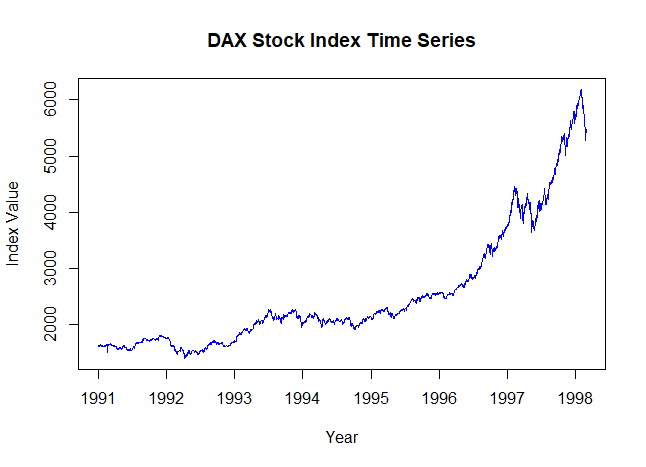
\includegraphics[width=0.8\textwidth]{Rplot03.png}
        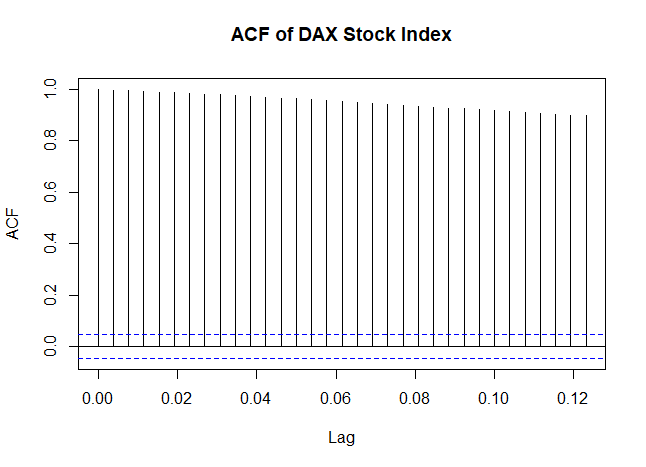
\includegraphics[width=0.8\textwidth]{Rplot04.png}
        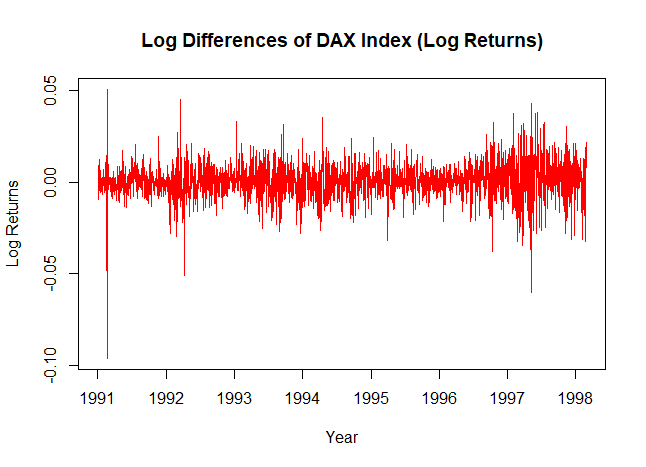
\includegraphics[width=0.8\textwidth]{Rplot05.png}
    \end{center}
    Some observations for the DAX stock index time series plot; visually, we can see that
    there is a general upward trend with some fluctuations. The ACF plot shows that there is
    a significant correlation at lag 1, followed by a gradual, slow decay, which means that it
    may be following other process we have not covered yet. The log returns plot shows that 
    the data revolves around 0, which is a good sign for stationarity.
    \end{enumerate} 
    \item
    \begin{enumerate}
    \item Given that the MA(1) process is defined as
    \[
        X_t = \mu_t + \epsilon_t + \theta \epsilon_{t-1}
    \]
    How we have to test whether the MA parameter is equal 
    to 0.
\begin{verbatim}
# Print the model summary
summary(ma1_model)

Call:
arima(x = nickel, order = c(0, 0, 1))

Coefficients:
            ma1  intercept
        0.2260     4.6223
s.e.  0.1099     0.0277

sigma^2 estimated as 0.03857:  
log likelihood = 15.63,  aic = -25.26

# Extract MA(1) coefficient and its standard error
theta_hat <- ma1_model$coef["ma1"]
se_theta <- sqrt(ma1_model$var.coef["ma1", "ma1"])

# Compute t-statistic
t_value <- theta_hat / se_theta

# Compute p-value (two-tailed test)
p_value <- 2 * (1 - pnorm(abs(t_value)))

# Print results
t_value
    ma1 
2.05681 
p_value
    ma1 
0.03970446
\end{verbatim}
    The fitted model is $X_t = 4.6223 + \epsilon_t + 0.2260 \epsilon_{t-1}$.
    Since the p-value is less than 0.05, we reject the null hypothesis that the MA parameter is equal to 0.
    
    \item The portmanteau test checks whether the residuals
    from our fitted MA(1) model behave like white noise, meaning they are uncorrelated.
    We can use the Box-Ljung test to check this.
\begin{verbatim}
# Perform the Box-Ljung test
Box.test(ma1_model$residuals, lag = 10, type = "Ljung-Box")

library(forecast)
checkresiduals(ma1_model)

Ljung-Box test

data:  Residuals from ARIMA(0,0,1) with non-zero mean
Q* = 2.5221, df = 5, p-value =
0.7732

Model df: 1.   Total lags used: 6
\end{verbatim}
    Since the p-value is greater than 0.05, we fail to reject the null hypothesis that the residuals are uncorrelated.
    \item If the 75th value is missing, we can forecast it using the fitted
    MA(1) model.
    \[
        X_{75} = 4.6223 + \epsilon_{75} + 0.2260 \epsilon_{74}
    \]
    Now we can extract the last residuals
\begin{verbatim}
# Extract last residual
epsilon_74 <- residuals(ma1_model)[74]

# Compute forecast
X_75_hat <- 4.6223 + (0.2260 * epsilon_74)
X_75_hat
[1] 4.545646
\end{verbatim}
    The forecasted value for $X_{75}$ is 4.545646.
    The standard deviation of the forecast is given by
    \[
        \sigma_{\text{forecast}} = \sqrt{\hat{\sigma}^2} \sqrt{1 + \theta^2}
    \]
    From the model, we have 
    \[
        \hat{\sigma}^2 = 0.03857
    \]
    \[
        \theta = 0.2260
    \]
    So we can calculate the standard deviation of the forecast.
    \[
        \sigma_{\text{forecast}} = \sqrt{0.03857} \sqrt{1 + 0.2260^2} = 0.2013455
    \]
    The error in terms of standard deviations is given by
    \[
        Z = \frac{X_{75} - X_{75}^{\text{forecast}}}{\sigma_{\text{forecast}}}
        = \frac{4.3 - 4.545646}{0.2013455} = -1.220022
    \]
    Since $|Z| < 2$, the forecast is within the 95\% confidence interval.

    \item First we fit an AR(1) model to the data.
\begin{verbatim}
ar1_model <- arima(nickel, order = c(1, 0, 0))

# Print model summary
summary(ar1_model)

Call:
arima(x = nickel, order = c(1, 0, 0))

Coefficients:
            ar1  intercept
        0.2363     4.6221
s.e.  0.1139     0.0295

sigma^2 estimated as 0.03845:  
log likelihood = 15.74,  aic = -25.47
\end{verbatim}
    Then we forecast for the 2nd and 3rd values after the end of
    the series.
\begin{verbatim}
# Forecast 2 steps ahead
ar1_forecast <- predict(ar1_model, n.ahead = 3)

# Print forecasted values
ar1_forecast$pred
Time Series:
Start = c(26, 1) 
End = c(26, 3) 
Frequency = 3 
[1] 4.545956 4.604083 4.617820
\end{verbatim} 
    Now we check if the residuals are white noise.
\begin{verbatim}
# Perform Ljung-Box test on AR(1) residuals
Box.test(ar1_model$residuals, lag = 10, type = "Ljung-Box")

Box-Ljung test

data:  ar1_model$residuals
X-squared = 7.1631, df = 10, p-value = 0.71
\end{verbatim}
    Since the p-value is greater than 0.05, 
    we fail to reject the null hypothesis that the 
    residuals are white noise.
    \end{enumerate}
    \item The given time series model is
    \[
        y_t = \mu + \phi(y_{t-1} - \mu) + \varepsilon_t
    \]
    The 
\end{enumerate}
\end{document}
